\documentclass{article}
\usepackage[margin=1in]{geometry}
\usepackage{siunitx}
\usepackage{array}
\usepackage{booktabs}
\usepackage{hyperref}
\usepackage{graphicx}
\usepackage{amsmath}

\begin{document}
\author{Sachith Dunatunga}
\title{16.930 PS4}
\maketitle

\section{Q1}
Surprisingly, the answer is provided in the reference material\cite{nguyen}.
The choice of $\tau$ which reduces to the regular DG method is given by
\begin{align}
\tau = \frac{1}{2} \left( | \mathbf{c} \cdot \mathbf{n} | + \mathbf{c} \cdot \mathbf{n} \right).
\end{align}

\section{Code}
The code is available at \url{http://github.com/neocpp89/16.930-ps4} and should be attached as well.
Most of the changes are contained to the hdg subdirectory.

A couple of problems I am aware of:
\begin{itemize}
\item Inhomogenous Dirichlet BCs don't seem to work (value is set on the nodes, but it doesn't propagate inside the domain).
I just removed the boundary portions of the matrix (assuming gd = 0) to allow the simulation to proceed.
\item I originally followed the notes and the reference material\cite{nguyen}, which use a formulation where $\mathbf{q} = \kappa \nabla u$ instead of $\mathbf{q} = \nabla u$ as requested. The code has been hastily converted since I only recently realized this may be an issue, but my primary test case uses $\kappa = 1$ so I may not have gotten all of it.
\item Distmesh seems to get stuck and can't create the structured mesh at times (keeps flipping a line across a quad).
It succeeds most of the time, but if it fails I have to interrupt and try again.
\end{itemize}

\section{Convergence plots for Structured Mesh}
% I am sorry about this, but I realized too late that I followed the notes a bit too closely and subsequently $\mathbf{q}$ approximates $\kappa \nabla u$ instead of $\nabla u$.
% Happily, this does not affect this test in particular (since $\kappa = 1$).
% The postprocessing also assumes $\kappa = 1$, since I did not want to modify the function signature, so it truly is applied on the gradient of $u$.

% The branch `grad-u' at \url{http://github.com/neocpp89/16.930-ps4} implements the version requested, but I am slightly dubious of the results.

In figure \ref{fig:cs} we see the expected convergence behavior of order p+1 for u when selecting $\tau = 1$ or $1/h$.
However, the rate drops to order p for $\tau = h$.

Interestingly, we see the expected convergence behaviors for $q_x$ and $q_y$ when selecting $\tau = 1$ or $\tau = h$, but the rate drops to order p for $\tau = 1/h$.

Since the postprocessing step relies on the order of $\mathbf{q}$ and $u$, it then makes sense that $\tau = 1$ results in a p+2 convergence rate for $u^*$. I was surprised that $\tau = h$ also had this p+2 rate (since u was order p), but I was not surprised that $\tau = 1/h$ would result in staying at order p+1 for $u^*$.

\begin{figure}
\centering
\begin{tabular}{c c c}
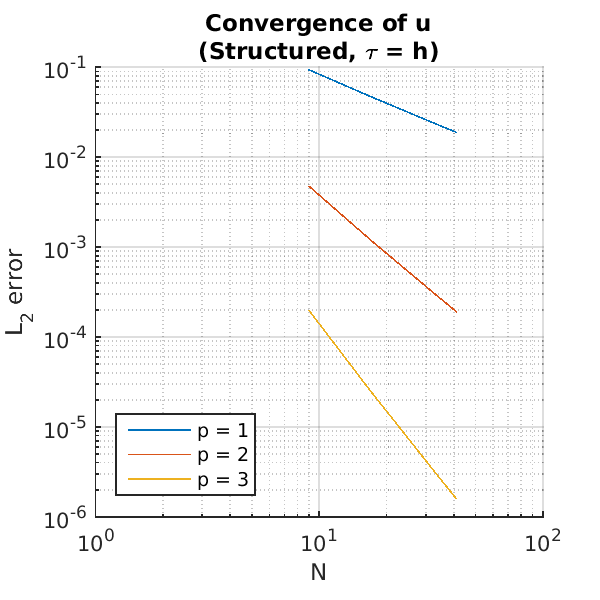
\includegraphics[scale=0.5]{cs_1.png} & 
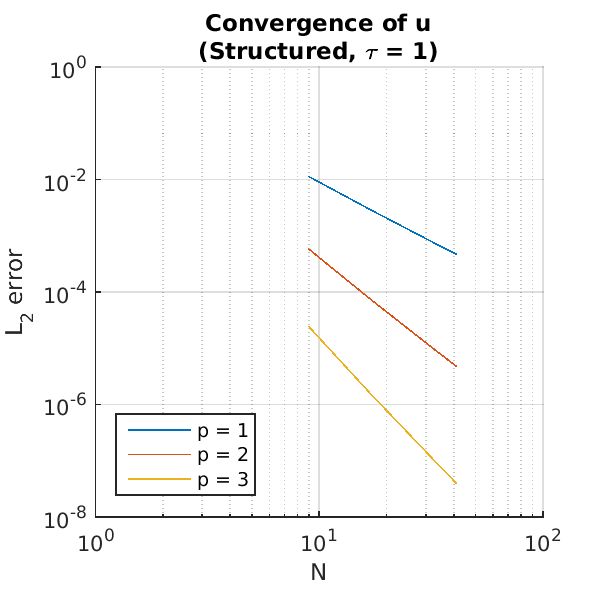
\includegraphics[scale=0.5]{cs_2.png} & 
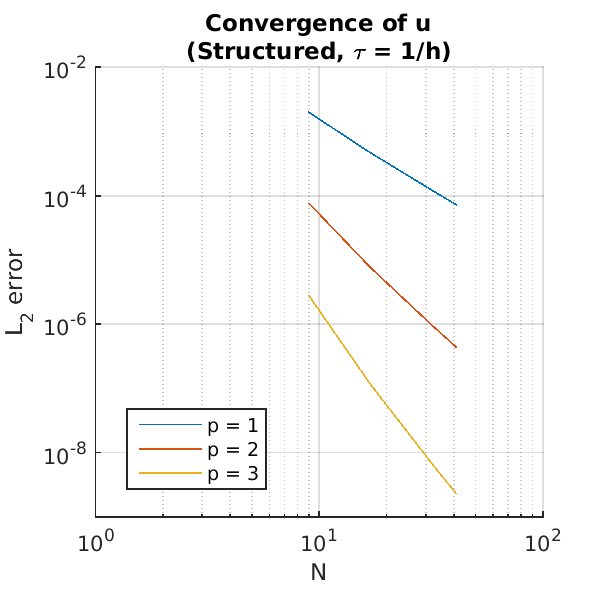
\includegraphics[scale=0.5]{cs_3.png} \\
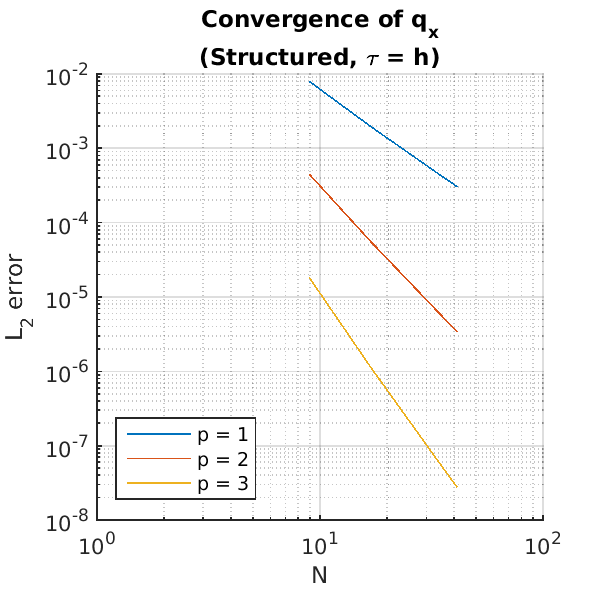
\includegraphics[scale=0.5]{csqx_1.png} & 
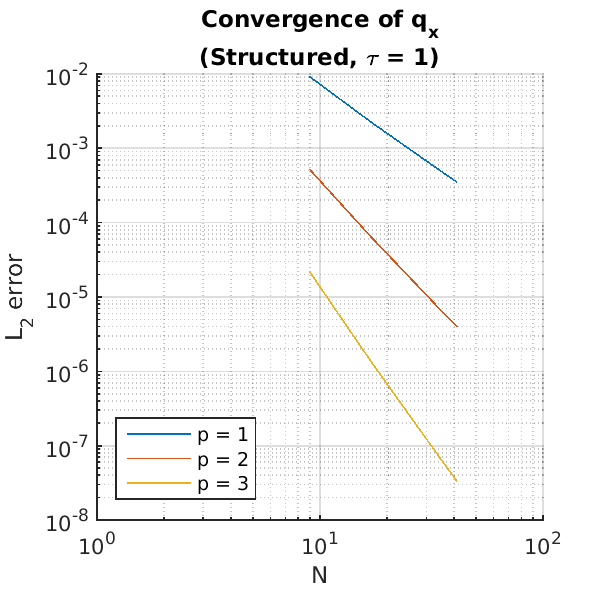
\includegraphics[scale=0.5]{csqx_2.png} & 
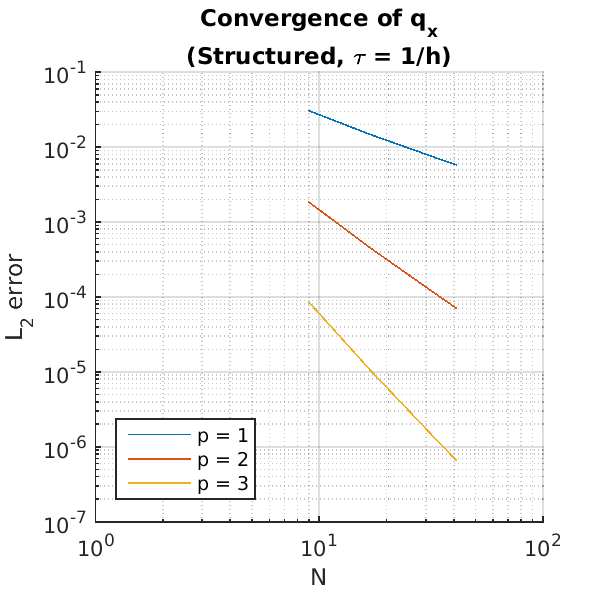
\includegraphics[scale=0.5]{csqx_3.png} \\
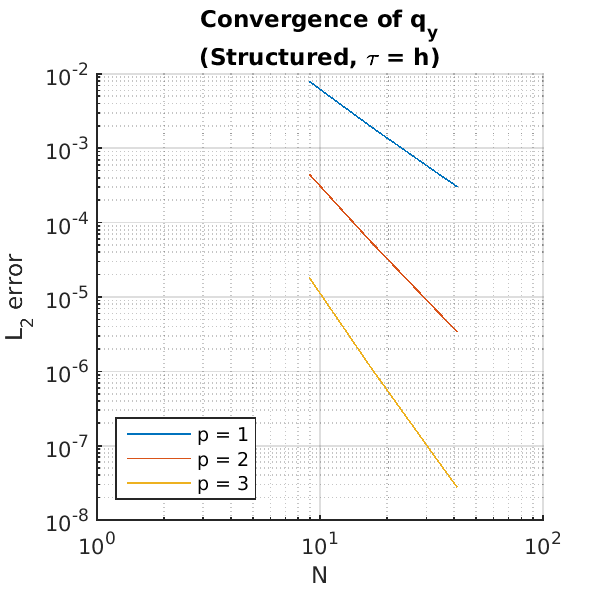
\includegraphics[scale=0.5]{csqy_1.png} & 
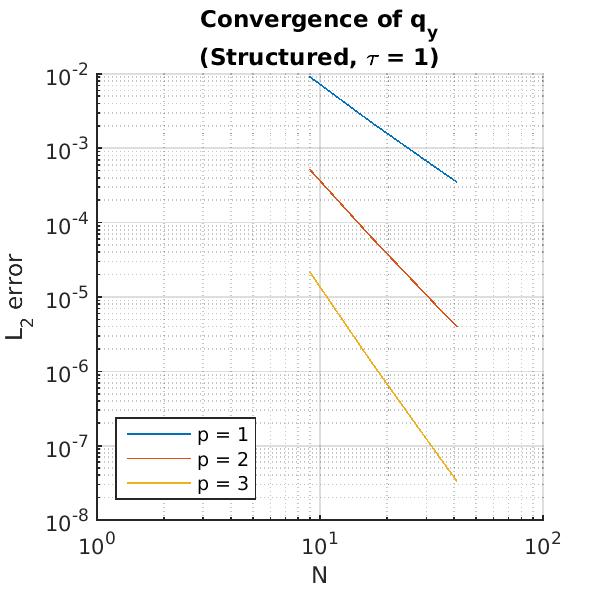
\includegraphics[scale=0.5]{csqy_2.png} & 
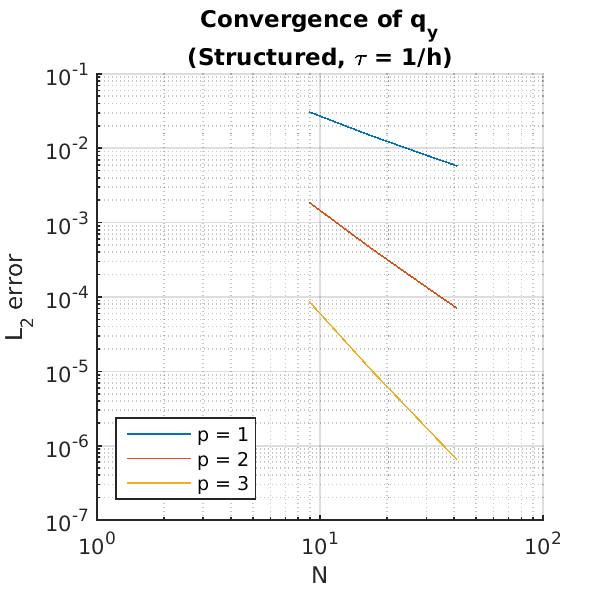
\includegraphics[scale=0.5]{csqy_3.png} \\
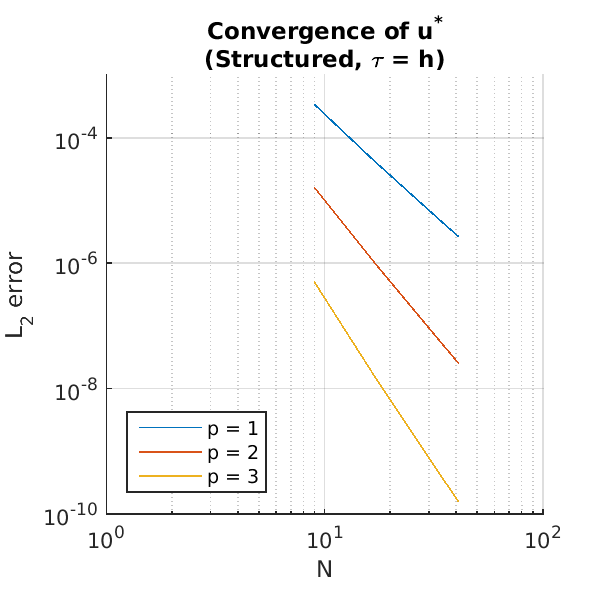
\includegraphics[scale=0.5]{cspp_1.png} & 
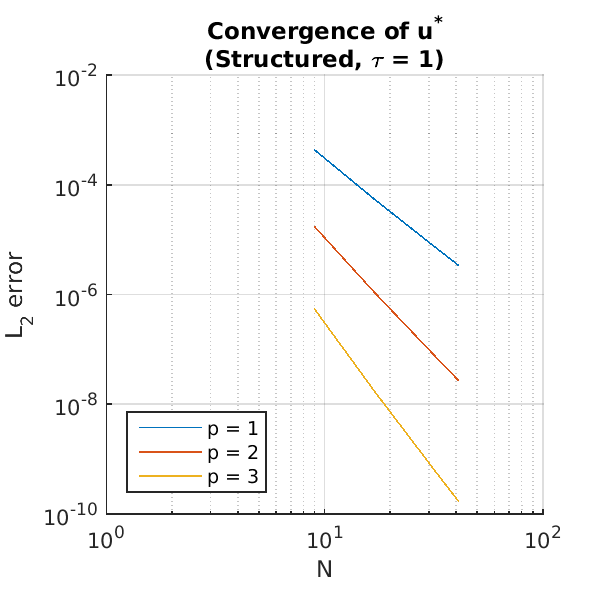
\includegraphics[scale=0.5]{cspp_2.png} & 
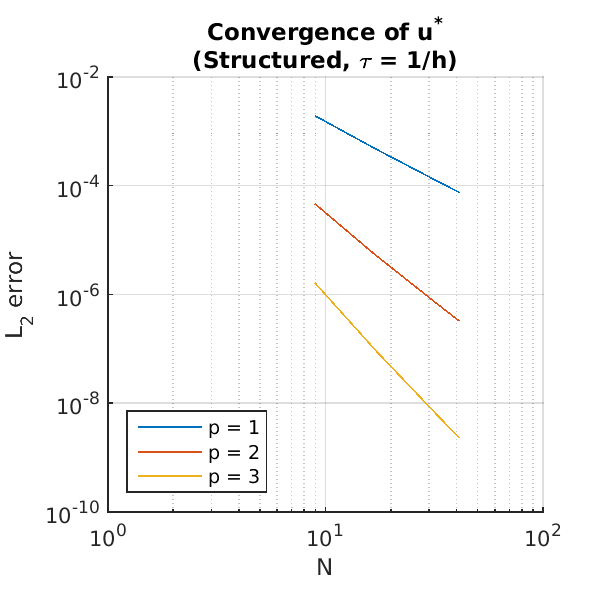
\includegraphics[scale=0.5]{cspp_3.png}
\end{tabular}
\caption{Convergence plots on the structured mesh. We have the stabilizations $\tau = h, 1, 1/h$ from left to right. The variables we compare are $u, q_x, q_y, u^*$ from top to bottom. We only get good convergence for everything when $\tau = 1$.}
\label{fig:cs}
\end{figure}

I did not have time to convert this to a proper table, but doing a linear fit of the last couple points confirms our code is working for the diffusion case.
I went out to 40 elements in addition to the specified 8, 16, and 32 sizes (convergence was higher than I expected with just the 3 meshes, but it appears to have been a transient effect, since the rate went back down by adding the even finer mesh).
The series below includes this mesh with n=40.
\begin{verbatim}
u
h - Order 1 has rate -1.02711.
h - Order 2 has rate -2.0551.
h - Order 3 has rate -3.08317.
1 - Order 1 has rate -2.04695.
1 - Order 2 has rate -3.07596.
1 - Order 3 has rate -4.10484.
1/h - Order 1 has rate -2.06656.
1/h - Order 2 has rate -3.13457.
1/h - Order 3 has rate -4.25809.
qx
h - Order 1 has rate -2.05846.
h - Order 2 has rate -3.08746.
h - Order 3 has rate -4.11365.
1 - Order 1 has rate -2.06695.
1 - Order 2 has rate -3.09276.
1 - Order 3 has rate -4.12155.
1/h - Order 1 has rate -1.03401.
1/h - Order 2 has rate -2.05983.
1/h - Order 3 has rate -3.08649.
qy
h - Order 1 has rate -2.05846.
h - Order 2 has rate -3.08746.
h - Order 3 has rate -4.11365.
1 - Order 1 has rate -2.06695.
1 - Order 2 has rate -3.09276.
1 - Order 3 has rate -4.12156.
1/h - Order 1 has rate -1.03401.
1/h - Order 2 has rate -2.05983.
1/h - Order 3 has rate -3.08649.
u*
h - Order 1 has rate -3.08705.
h - Order 2 has rate -4.11205.
h - Order 3 has rate -5.14057.
1 - Order 1 has rate -3.08851.
1 - Order 2 has rate -4.11603.
1 - Order 3 has rate -5.1444.
1/h - Order 1 has rate -2.05619.
1/h - Order 2 has rate -3.09672.
1/h - Order 3 has rate -4.12233.
\end{verbatim}

\clearpage

\section{Unstructured Mesh}

In figure \ref{fig:um} we see the meshes used.
Since they are generated by distmesh, they may change from run to run.

\begin{figure}[!ht]
\centering
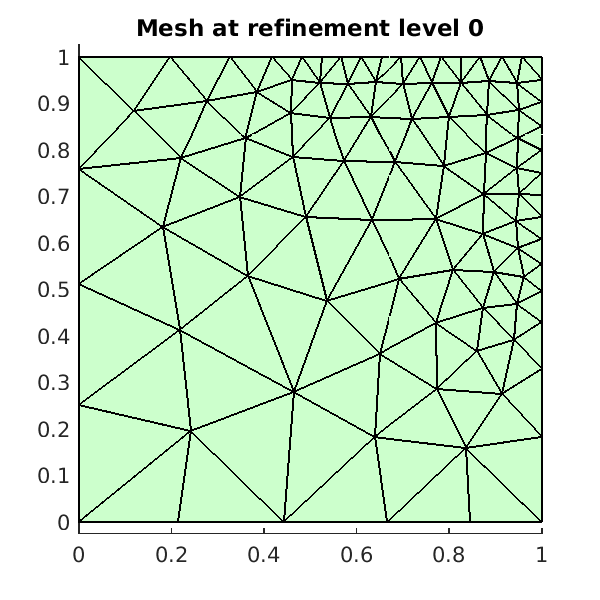
\includegraphics[scale=0.5]{um_1.png}
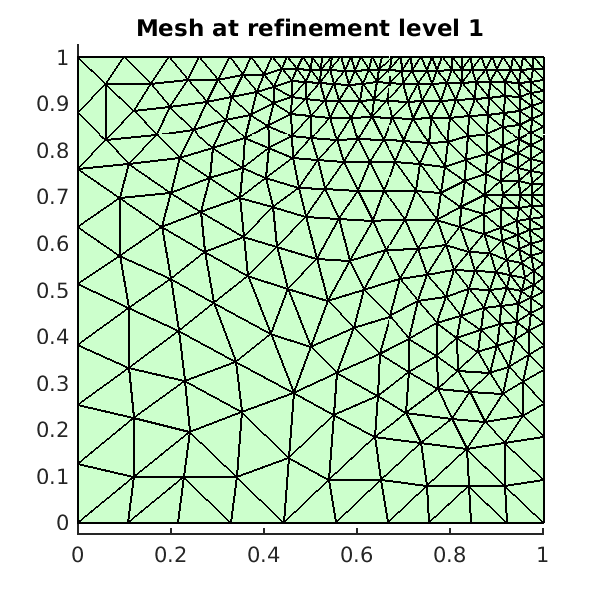
\includegraphics[scale=0.5]{um_2.png}
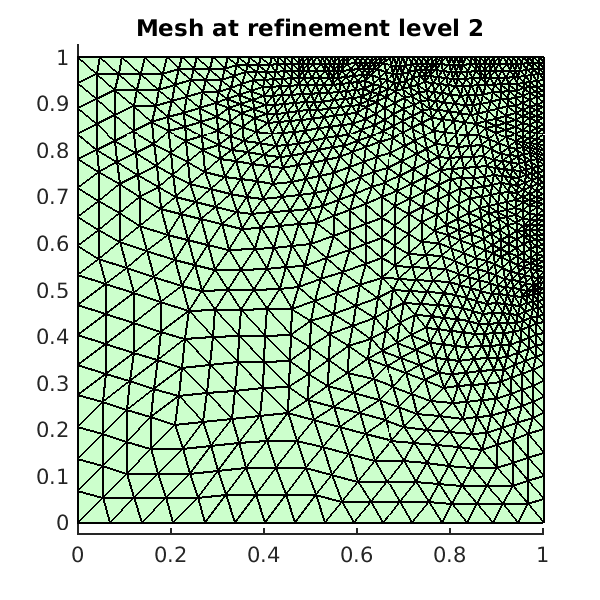
\includegraphics[scale=0.5]{um_3.png}
\caption{The mesh generated, and refinements thereof. Elements are more clustered towards boundaries where layers will begin to form. The order of elements in the mesh can be changed and is used for separate runs as well as postproceseing.}
\end{figure}

Perhaps unsurprisingly, when diffusion dominates, the boundary layer is large and is easily captured even by the coarsest mesh.
Purely relying on the visualization we can't tell the difference between the pre and postprocessed solutions and neither can we notice a difference between the p=1 and p=3 elements, as shown in figure \ref{fig:u100} and \ref{fig:ustar100}.

\begin{figure}[!ht]
\centering
\begin{tabular}{c c}
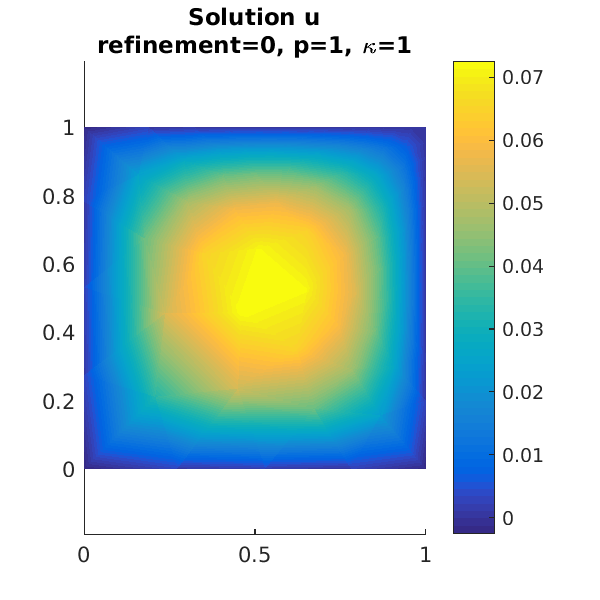
\includegraphics[scale=0.7]{umu_111.png} & 
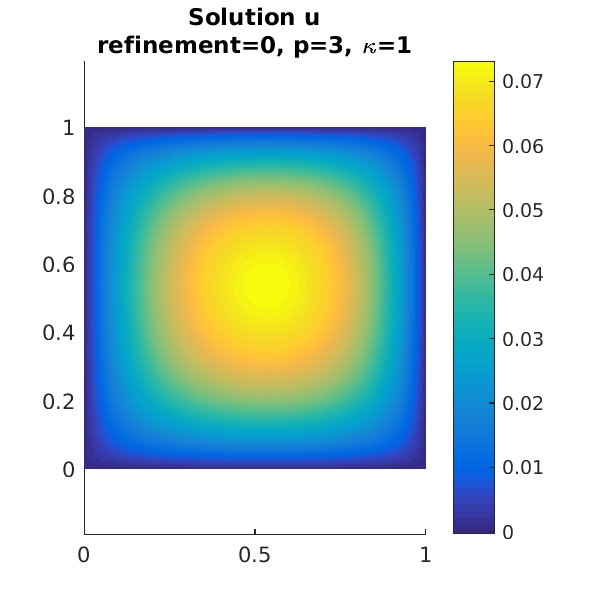
\includegraphics[scale=0.7]{umu_211.png} \\
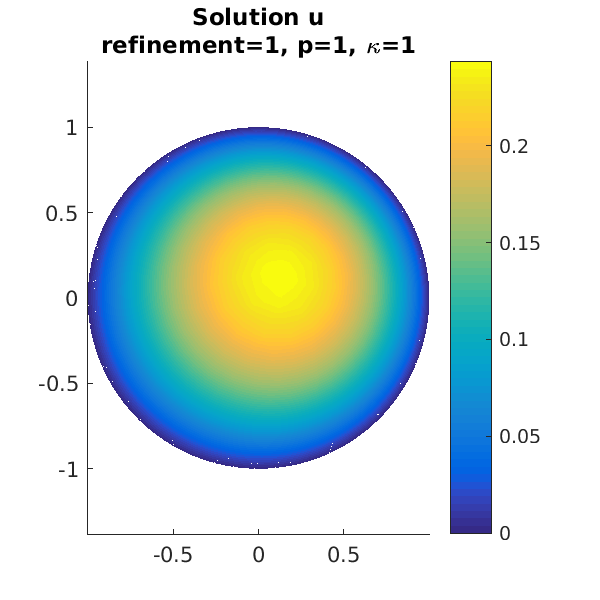
\includegraphics[scale=0.7]{umu_121.png} & 
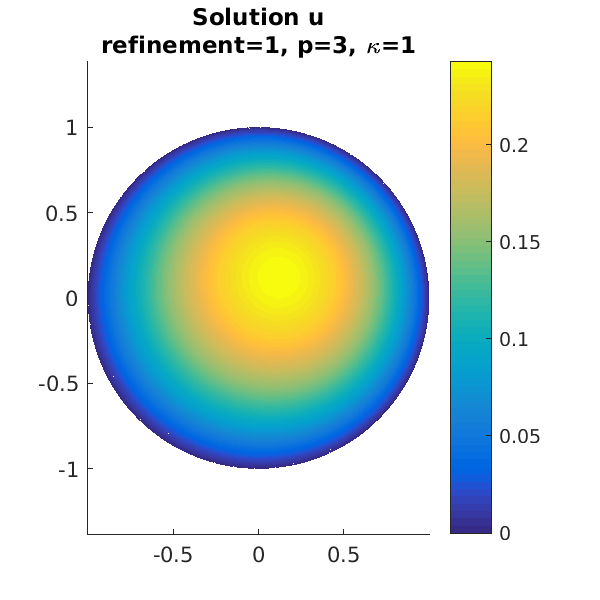
\includegraphics[scale=0.7]{umu_221.png} \\
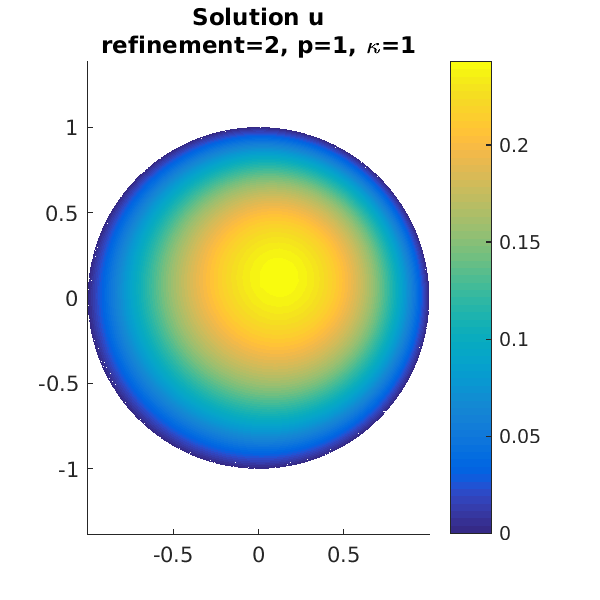
\includegraphics[scale=0.7]{umu_131.png} & 
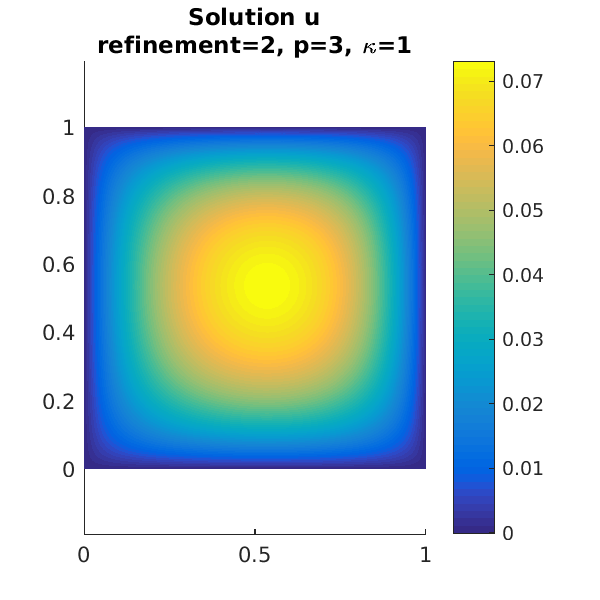
\includegraphics[scale=0.7]{umu_231.png}
\end{tabular}
\caption{The diffusion-dominated case with $\kappa = 1$. Solutions from the p=1 elements are shown on the left while the p=3 elements are on the right.}
\label{fig:u100}
\end{figure}

\begin{figure}[!ht]
\centering
\begin{tabular}{c c}
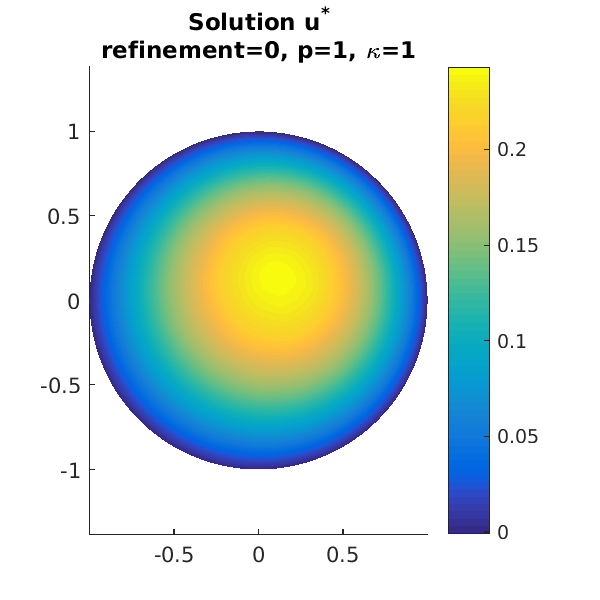
\includegraphics[scale=0.7]{umustar_111.png} &
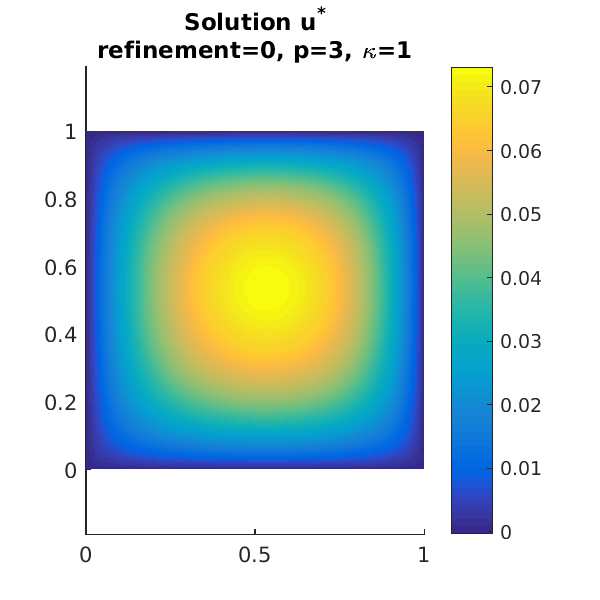
\includegraphics[scale=0.7]{umustar_211.png} \\
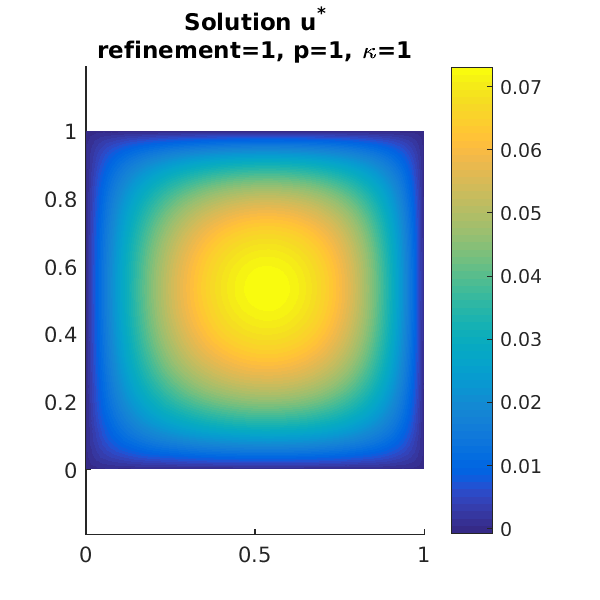
\includegraphics[scale=0.7]{umustar_121.png} &
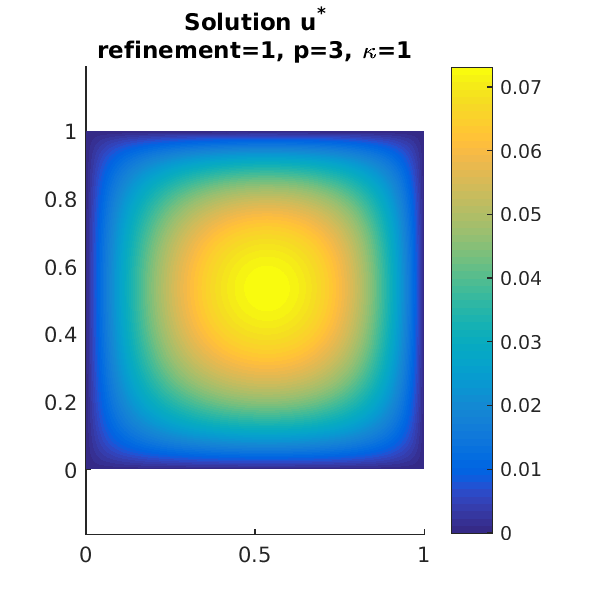
\includegraphics[scale=0.7]{umustar_221.png} \\
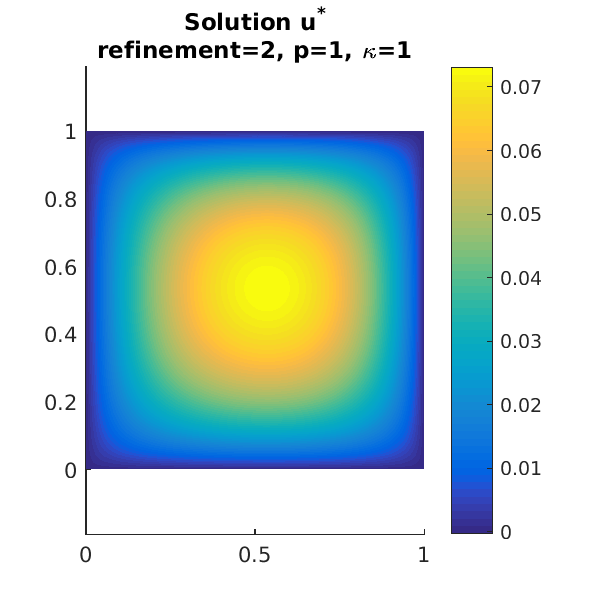
\includegraphics[scale=0.7]{umustar_131.png} &
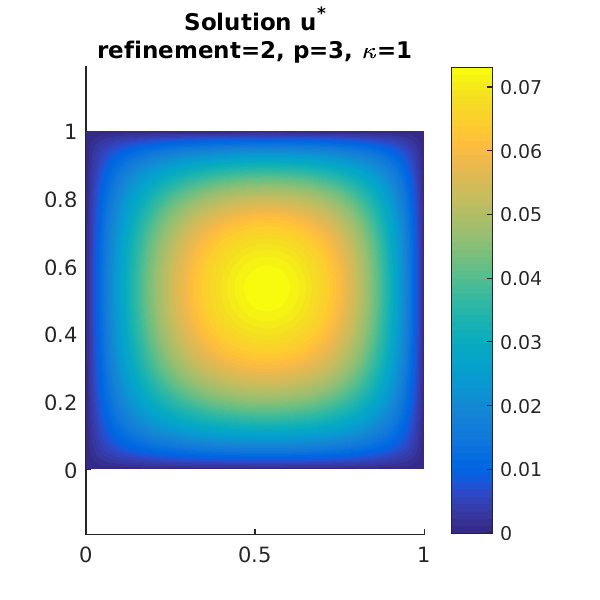
\includegraphics[scale=0.7]{umustar_231.png}
\end{tabular}
\caption{The diffusion-dominated case with $\kappa = 1$. Postprocessed solutions from the p=1 elements are shown on the left while the p=3 elements are on the right.}
\label{fig:ustar100}
\end{figure}

When convenction becomes more dominant, we start to see the effects of a boundary layer in the solution.
While at $\kappa = 0.1$ (c unchanged) the boundary layer in the solution still looks reasonable, we are able to see a difference now between refinement levels and between element orders. However, once the postprocessing is applied, it again becomes difficult to discern any difference between the simulations.

\begin{figure}[!ht]
\centering
\begin{tabular}{c c}
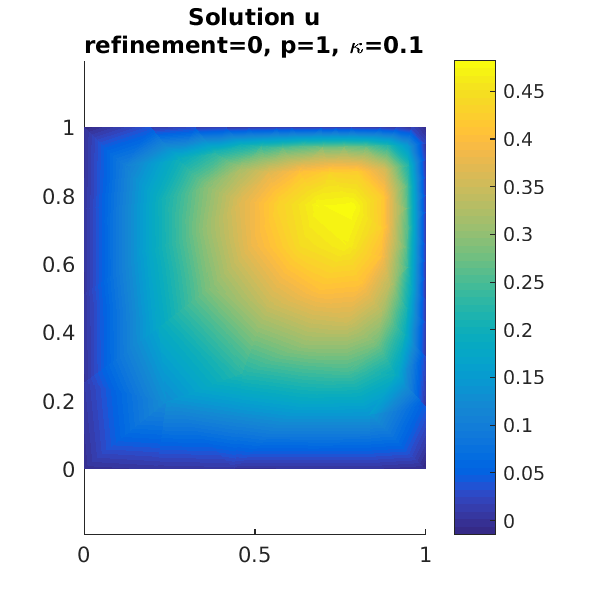
\includegraphics[scale=0.7]{umu_112.png} & 
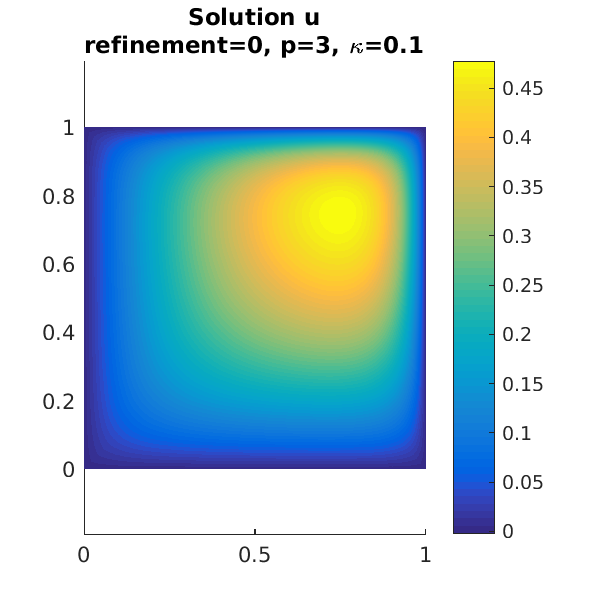
\includegraphics[scale=0.7]{umu_212.png} \\
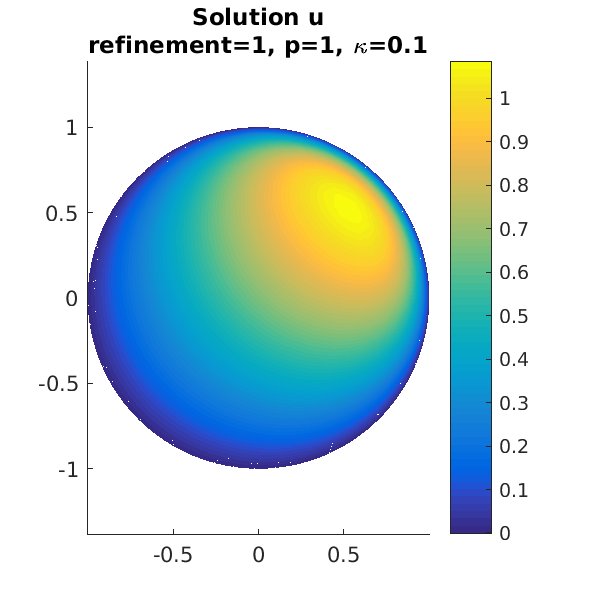
\includegraphics[scale=0.7]{umu_122.png} & 
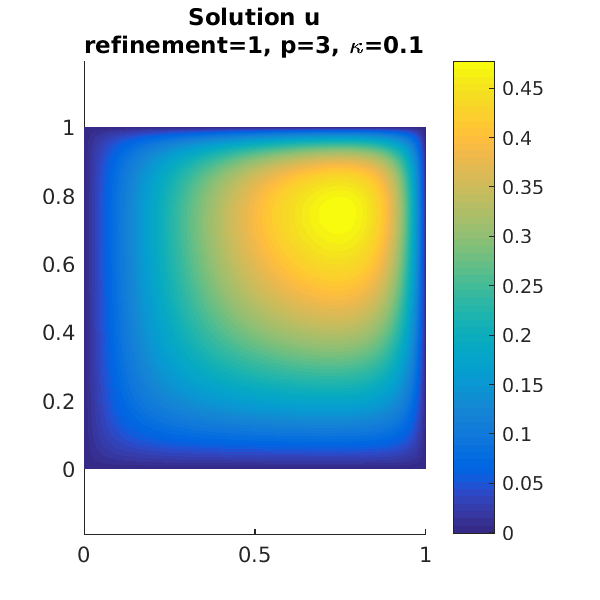
\includegraphics[scale=0.7]{umu_222.png} \\
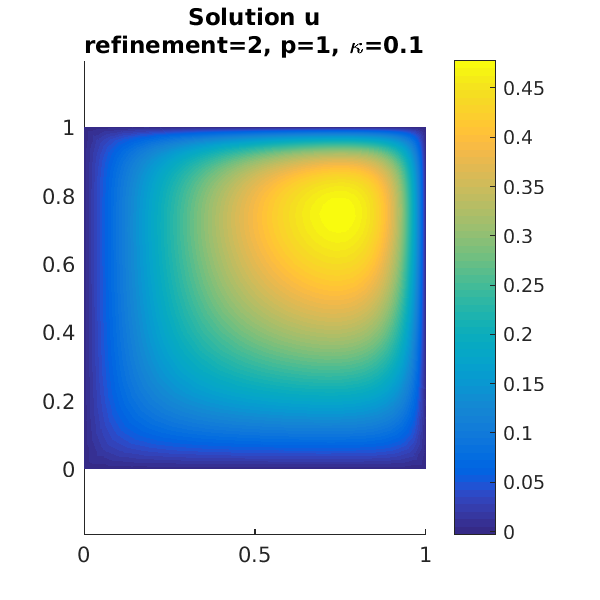
\includegraphics[scale=0.7]{umu_132.png} & 
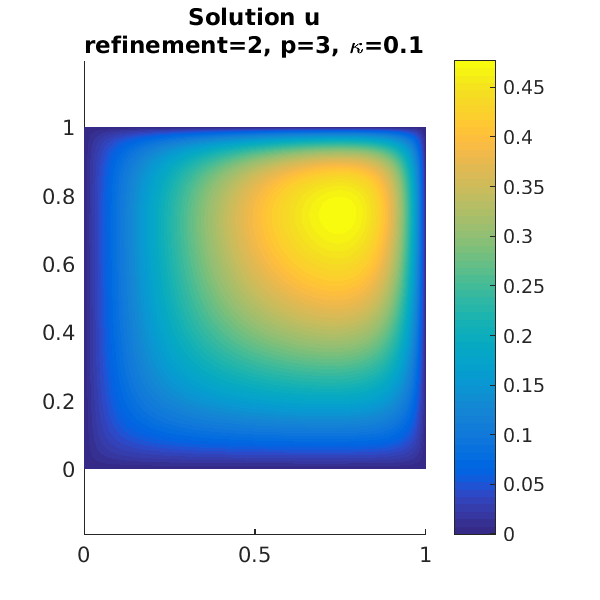
\includegraphics[scale=0.7]{umu_232.png}
\end{tabular}
\caption{The mixed case with $\kappa = 0.1$. Solutions from the p=1 elements are shown on the left while the p=3 elements are on the right.}
\label{fig:u100}
\end{figure}

\begin{figure}[!ht]
\centering
\begin{tabular}{c c}
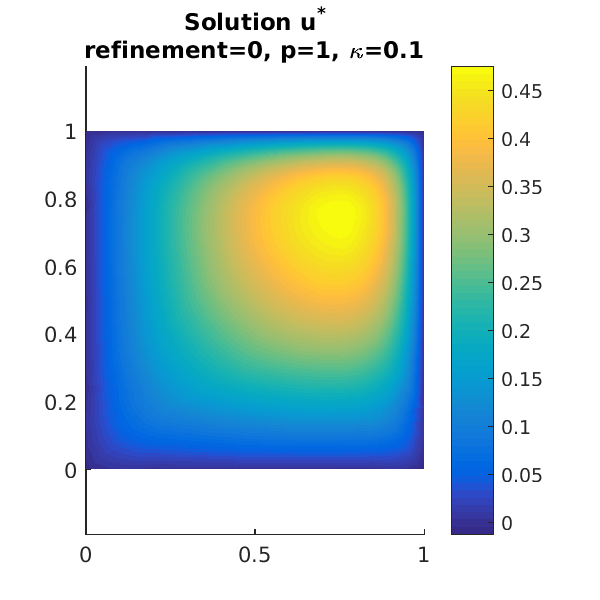
\includegraphics[scale=0.7]{umustar_112.png} &
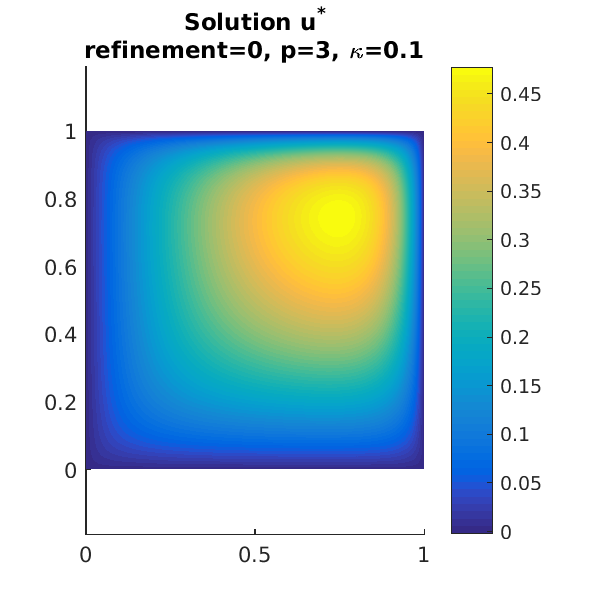
\includegraphics[scale=0.7]{umustar_212.png} \\
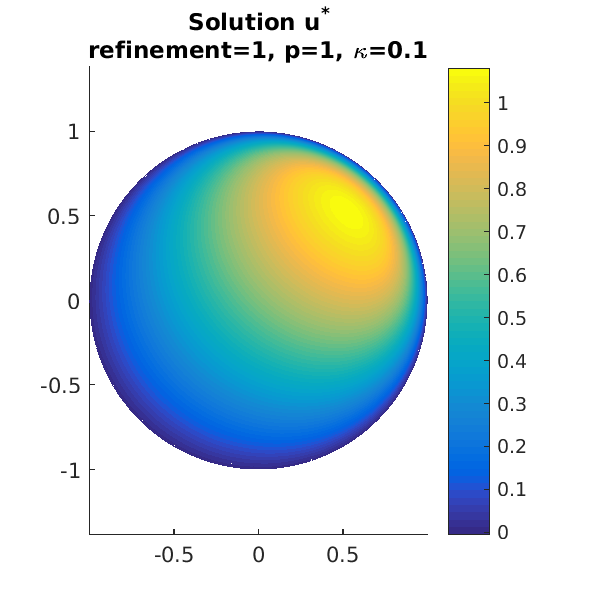
\includegraphics[scale=0.7]{umustar_122.png} &
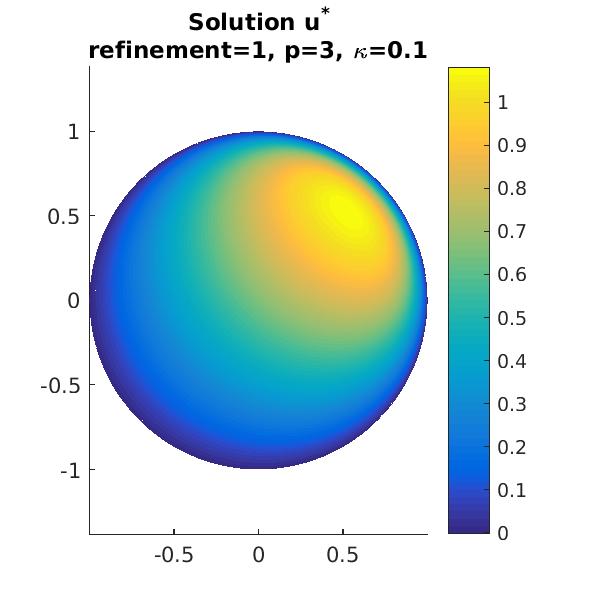
\includegraphics[scale=0.7]{umustar_222.png} \\
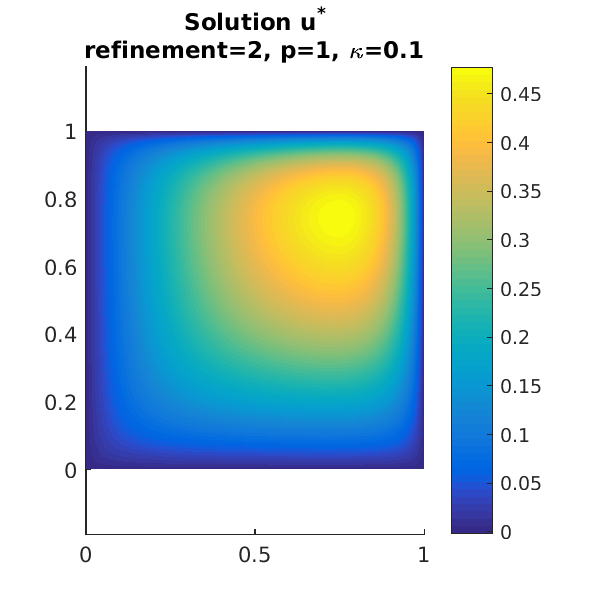
\includegraphics[scale=0.7]{umustar_132.png} &
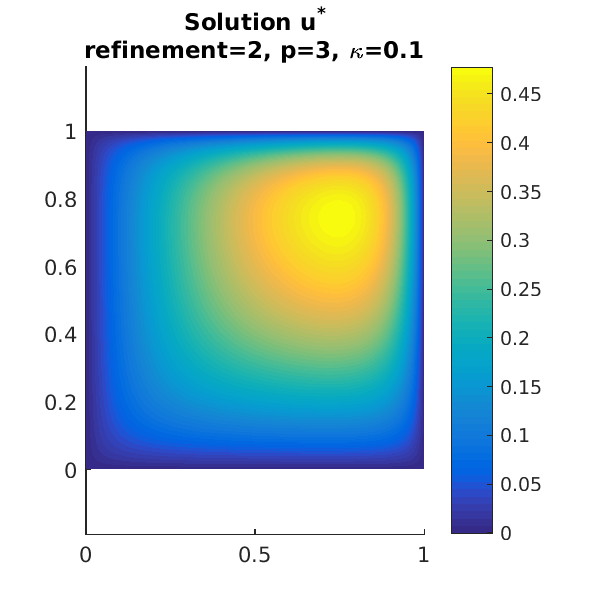
\includegraphics[scale=0.7]{umustar_232.png}
\end{tabular}
\caption{The mixed case with $\kappa = 0.1$. Postprocessed solutions from the p=1 elements are shown on the left while the p=3 elements are on the right.}
\label{fig:ustar100}
\end{figure}

In the convection-dominated case, we see a very clear boundary layer, which causes us to generate a poor solution when the mesh is coarse.
Reducing the element size until the boundary layer fits results in dramatic improvement.
We also noticed that the postprocessing does not seem to help in this case.
We suspect this is because the postprocessing step does not take into account any of the convection (only diffusion), and note that there is no dimensionless group relating the two in the postprocessing equations.
This is okay when the convection is swamped out anyways by diffusion, but it is probably not a good idea in a convection-dominated environment.

\begin{figure}[!ht]
\centering
\begin{tabular}{c c}
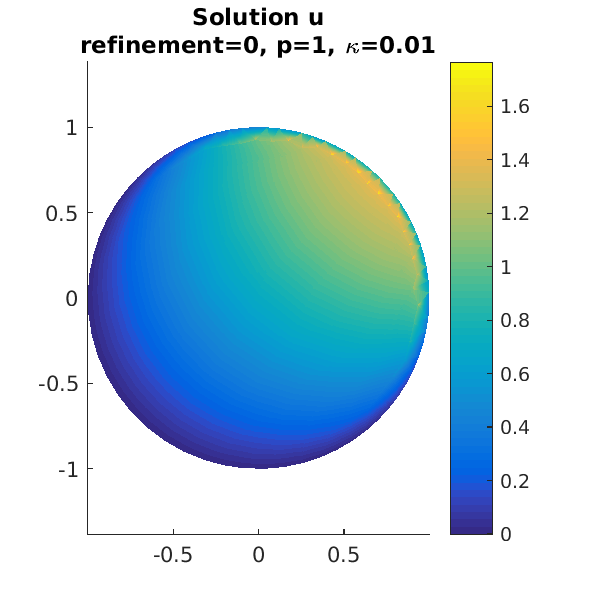
\includegraphics[scale=0.7]{umu_113.png} & 
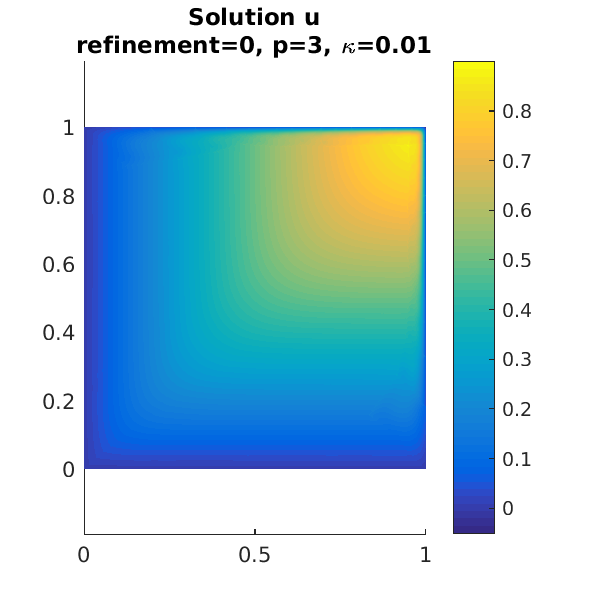
\includegraphics[scale=0.7]{umu_213.png} \\
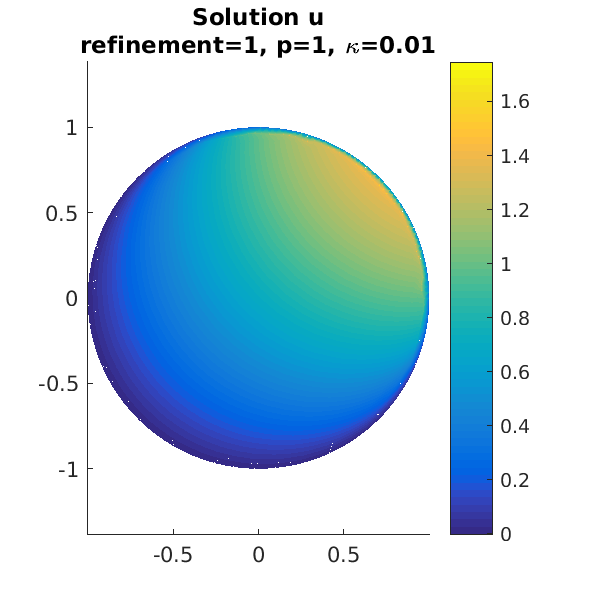
\includegraphics[scale=0.7]{umu_123.png} & 
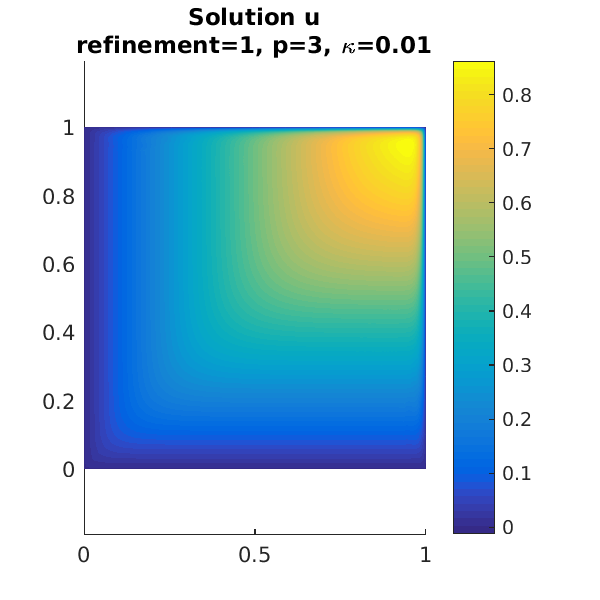
\includegraphics[scale=0.7]{umu_223.png} \\
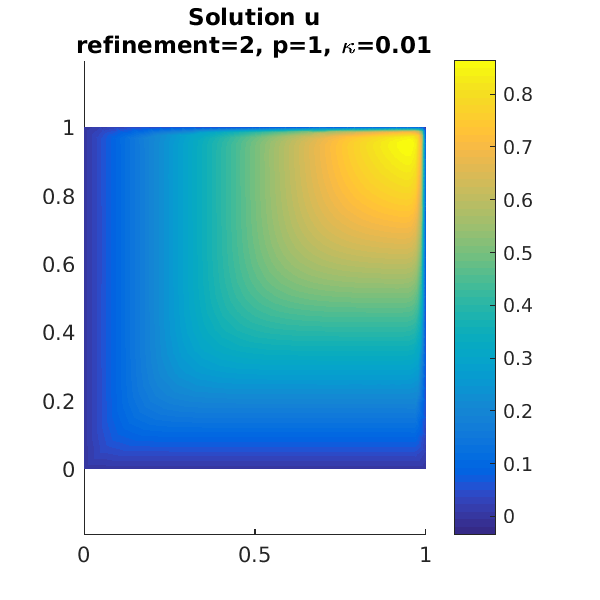
\includegraphics[scale=0.7]{umu_133.png} & 
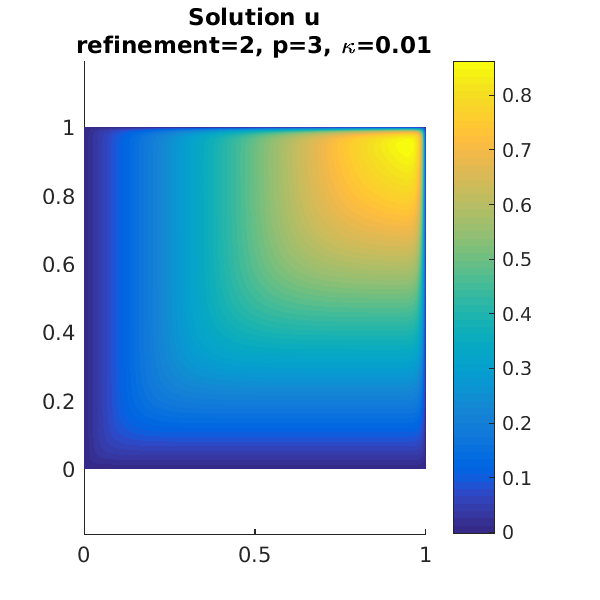
\includegraphics[scale=0.7]{umu_233.png}
\end{tabular}
\caption{The convection-dominated case with $\kappa = 0.01$. Solutions from the p=1 elements are shown on the left while the p=3 elements are on the right.}
\label{fig:u100}
\end{figure}

\begin{figure}[!ht]
\centering
\begin{tabular}{c c}
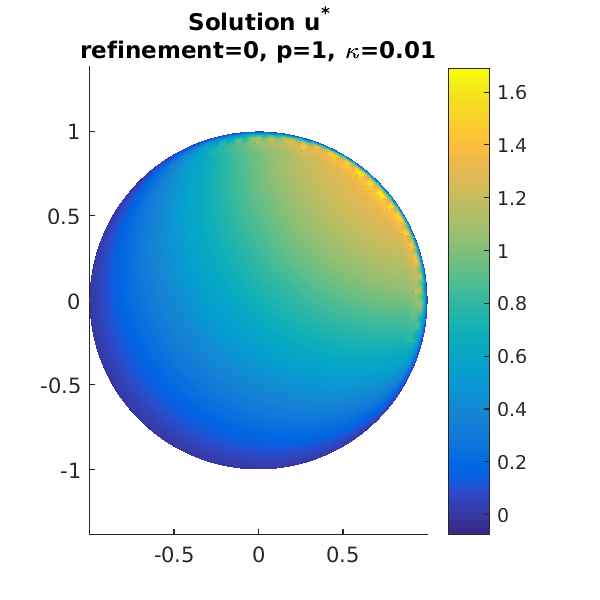
\includegraphics[scale=0.7]{umustar_113.png} &
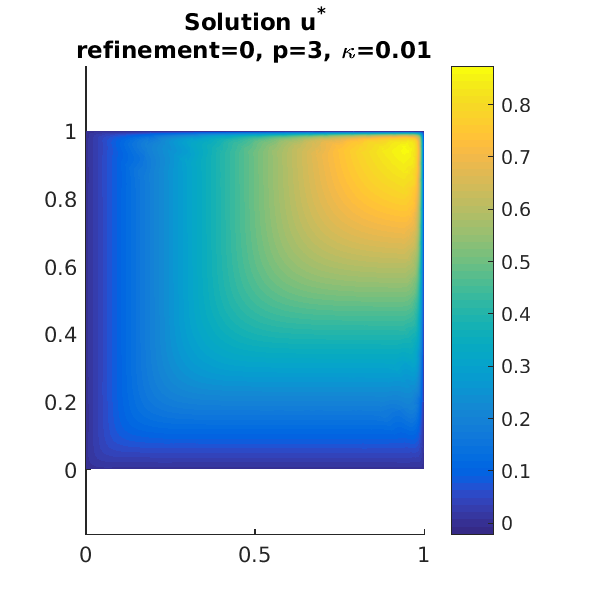
\includegraphics[scale=0.7]{umustar_213.png} \\
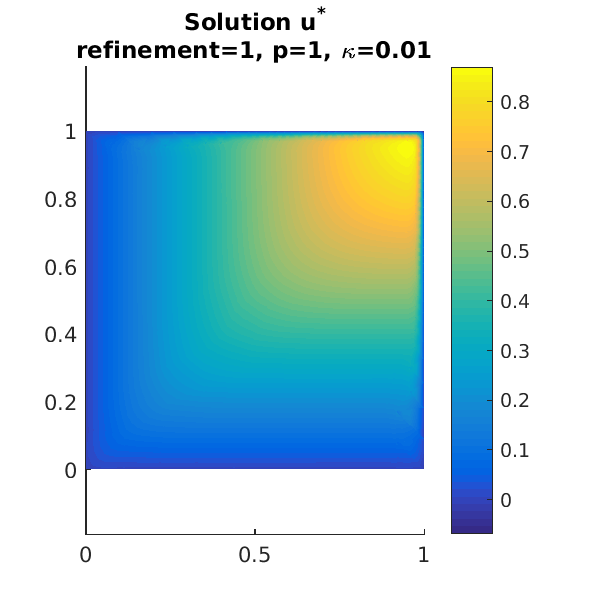
\includegraphics[scale=0.7]{umustar_123.png} &
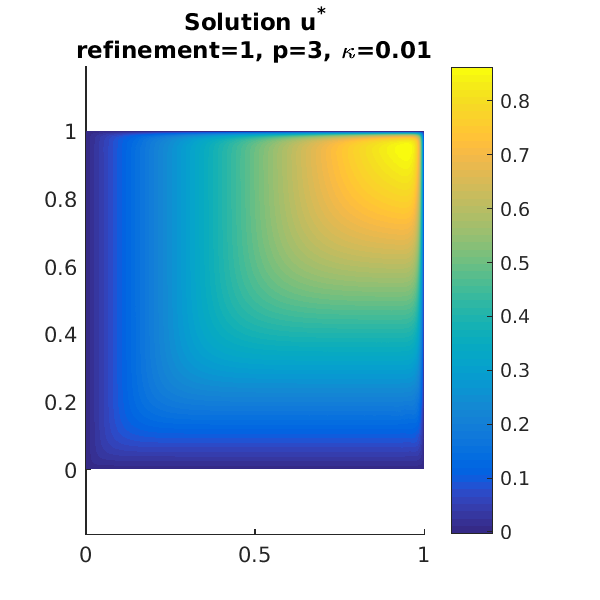
\includegraphics[scale=0.7]{umustar_223.png} \\
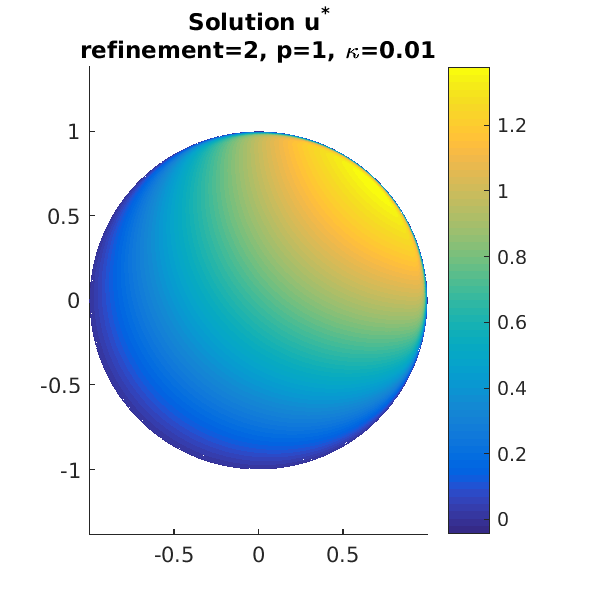
\includegraphics[scale=0.7]{umustar_133.png} &
\includegraphics[scale=0.7]{umustar_233.png}
\end{tabular}
\caption{The convection-dominated case with $\kappa = 0.01$. Postprocessed solutions from the p=1 elements are shown on the left while the p=3 elements are on the right.}
\label{fig:ustar100}
\end{figure}
\begin{thebibliography}{9}
\bibitem{nguyen}
N.C. Nguyen, J. Peraire, B. Cockburn
\textit{An implicit high-order hybridizable discontinuous Galerkin method for linear convection-diffusion equations}
Journal of Computational Physics, 228 (2009) 3232-3254
\end{thebibliography}

\end{document}
